\documentclass{article}
\usepackage{graphicx} % Required for inserting images
\usepackage[T1]{fontenc}
\usepackage[utf8]{inputenc}
\usepackage{hyperref}

\title{Izumi koji se bore protiv razvoja tehnologije za prepoznavanje lica}
\author{Anja Čolić}
\date{Jun 2023}
\newcommand{\profesor}{Profesor Dr. Sana Stojanović Đurđević}
\newcommand{\fakultet}{Matematički fakultet}


\begin{document}


\pagenumbering{gobble}

\maketitle

\begin{center}
\profesor
\end{center}


\newpage
\pagenumbering{arabic}
\renewcommand{\contentsname}{Sadržaj}
% Druga stranica - Sadržaj
\tableofcontents
\newpage

\





\maketitle

\section{Uvod}

Tehnologija prepoznavanja lica je biometrijska tehnologija koja koristi veštačku inteligenciju i algoritme mašinskog učenja kako bi identifikovala i verifikovala pojedince na osnovu njihovih karakteristika lica. 
\newline
\newline
Ova tehnologija je u poslednjoj deceniji brzo napredovala i sada se široko koristi.
Iako nudi mnoge potencijalne prednosti, u ovom radu ću razmotriti negativnu stranu iste i pokušati da odgovorim na pitanja da li je prikupljanje i korišćenje podataka o prepoznavanju lica moralno ispravno i da li se to može opravdati?
\newline
\newline
Dakle, cilj obrade ove teme je podizanje svesti o pravu na privatnost i zaštiti biometrijskih podataka, kao što je slika lica pojedinca.
\newpage

\section{Tehnologije i izumi}
\subsection{Specijalna maska}
Jedan primerak specijalne maske (Slika 1), koja se bori za privatnost pojedinca i protiv tehnologije prepoznavanja lica, delo je tehnologa Jip van Levenštajna. Levenštajnova veb stranica kaže da je ova maska formirana kao sočivo. Dizajnirana je da vas učini neprepoznatljivim za softver za prepoznavanje, dok vam i dalje omogućava da komunicirate sa drugim ljudima bez gubitka identiteta i izraza lica.

\begin{center}
\begin{minipage}{0.5\textwidth}
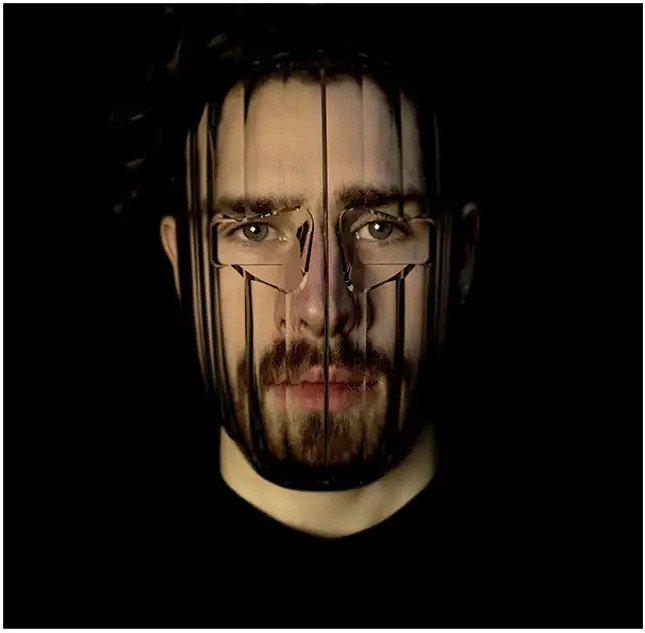
\includegraphics[width=\textwidth]{slika.jpg}
\end{minipage}

\vspace{0.5cm}

Slika 1: Maska Jip van Levenštajna
\end{center}

\subsection{Vizir/Naočare}
Još jedan izum koji podržava nauka dolazi iz laboratorije pri Nacionalnom institutu za informatiku u Japanu. Ovaj vizir koji podseća na naočare(Slika 2), ima ugrađene LED diode koje zaustavljaju prepoznavanje lica. Rade tako što reflektuju svetlo koje dolazi prema njima, što otežava prepoznavanje lica kamere koje se nalaze u blizini.


\begin{center}
\begin{minipage}{0.5\textwidth}
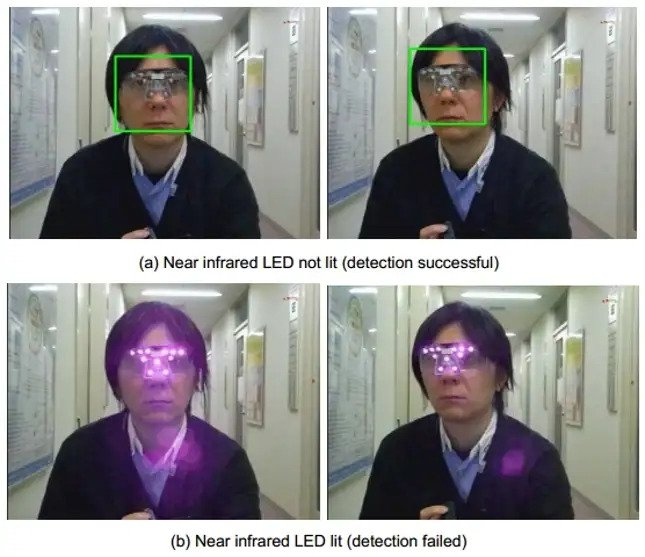
\includegraphics[width=\textwidth]{naocare.jpg}
\end{minipage}

\vspace{0.5cm}

Slika 2: Specijalne naočare, Nacionalni institut za Informatiku Japan
\end{center}


\subsection{Odeća}
Italijanski start-up Capable nudi svoju prvu kolekciju pletene odeće koja štiti korisnika od softvera za prepoznavanje lica (Slika 3), bez potrebe da pokrije lice maskom ili naočarama. Svaki odevni predmet ima šaru, poznatu kao „adversarial flatch“, koju su razvili AI algoritmi da zbuni softver za prepoznavanje lica u realnom vremenu i zaštiti privatnost korisnika. Kamera ili neće uspeti da identifikuje nosioca ili će misliti da je isti jedna od životinja ugrađena u obrazac (zebra, žirafa ili pas, između ostalih životinja). 

\begin{center}
\begin{minipage}{0.5\textwidth}
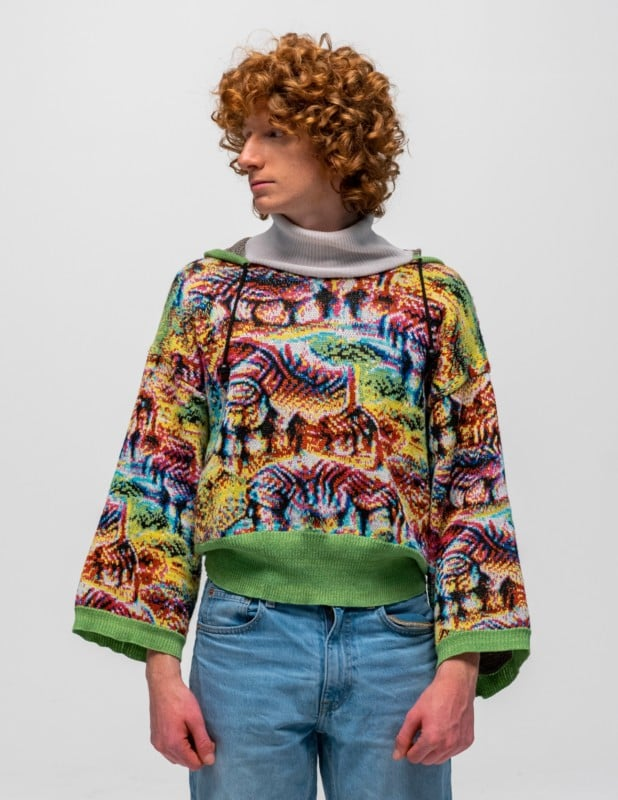
\includegraphics[width=\textwidth]{odeca2.jpg}
\end{minipage}

\vspace{0.5cm}

Slika 3: Specijalna kolekcija odeće brenda Capable
\end{center}

\subsection{Nosivi projektor za lice}
Projektor lica koji se može nositi prikazuje potpuno novo lice na vašem sopstvenom, pa samim tim otežava algoritmu da vas prepozna. Ovo je jedan od dizajna koji su 2017. godine napravili studenti sa Univerziteta umetnosti u Utrehtu. 


\begin{center}
\begin{minipage}{0.5\textwidth}
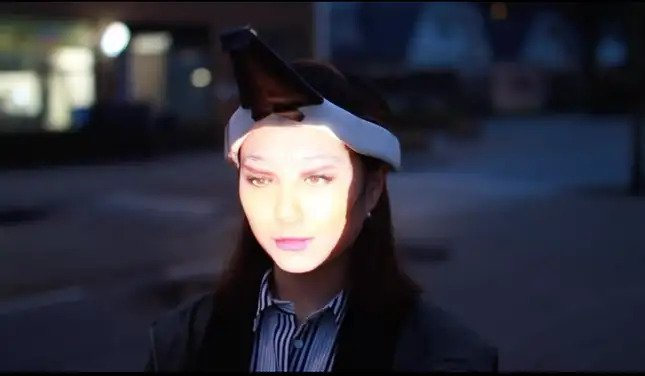
\includegraphics[width=\textwidth]{projektor.jpg}
\end{minipage}

\vspace{0.5cm}

Slika 4: Nosivi projektor za lice
\end{center}

\subsection{Šminka}
Nova studija sa Univerziteta Ben-Gurion u Negevu otkrila je da se obrasci šminke generisani softverom mogu koristiti za dosledno zaobilaženje softvera za prepoznavanje lica, pri čemu digitalno i fizički primenjena šminka zavara neke sisteme sa stopom uspeha 98 \%.
\newline
\newline
Međutim, oni nisu prvi koji su pokazali kako se šminka može koristiti za zavaravanje sistema za prepoznavanje lica. Projekat CV Dazzle umetnika Adama Harvija predstavio je mnogo izgleda šminke dizajniranih da prevari algoritme, inspirisane kamuflažom koja se koristila u Prvom svetskom ratu.

\begin{center}
\begin{minipage}{0.5\textwidth}
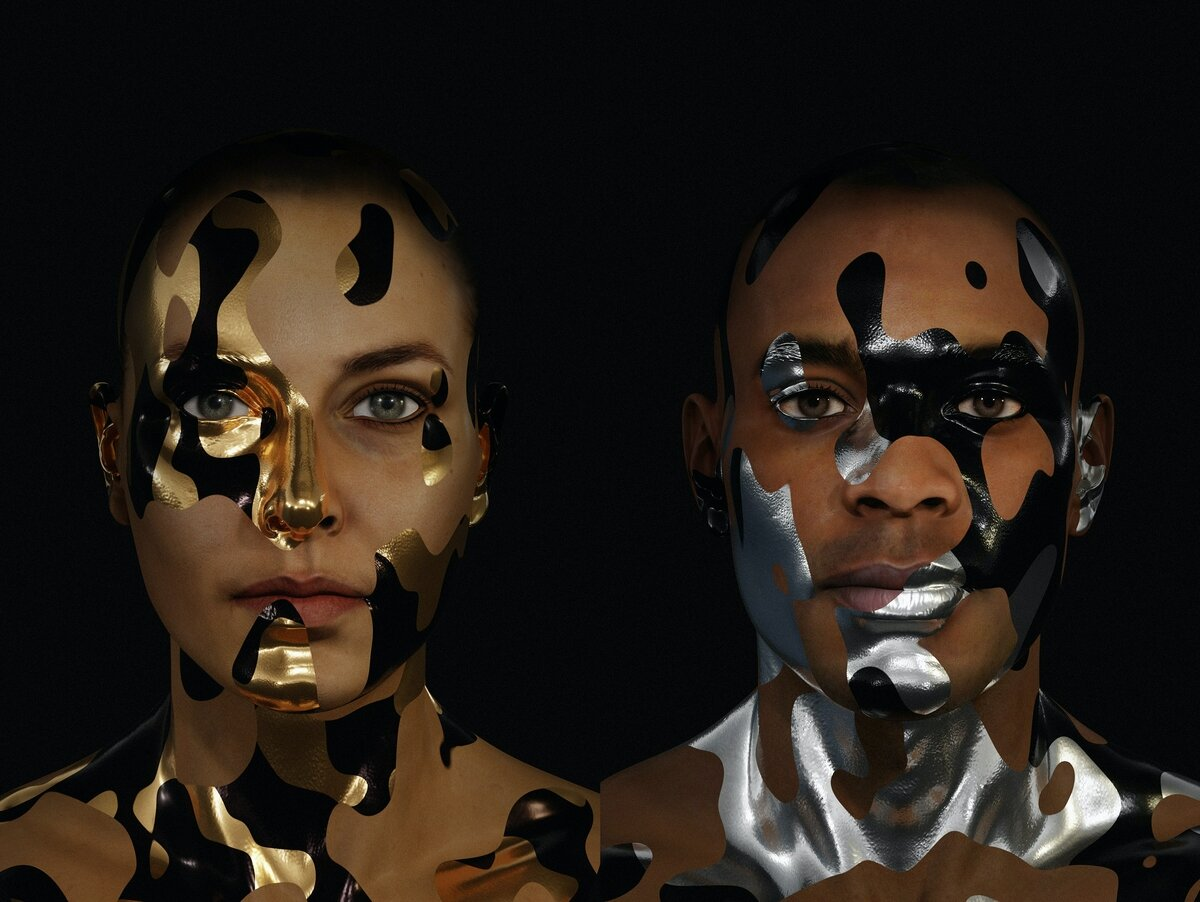
\includegraphics[width=\textwidth]{sminka2.jpg}
\end{minipage}

\vspace{0.5cm}

Slika 5: Primer šminke umetnika Adama Harvija iz 2020.
\end{center}

\section{Pitanje privatnosti i etike}

\subsection{Nedostatak informisanog pristanka i transparentnosti}

Privatnost je jedna od zabrinutosti kada je ova tehnologija u pitanju, uglavnom zbog nedostatka transparentnosti u vezi sa načinom na koji se informacije čuvaju i upravljaju. 
\newline
\newline
Godine 2020, Evropska komisija je zabranila tehnologiju prepoznavanja lica u javnim prostorima na period do pet godina kako bi izmenila svoj pravni okvir i uključila smernice o privatnosti i etičkoj zloupotrebi.
\newline
\newline
Brige oko privatnosti u vezi sa tehnologijom prepoznavanja lica odnose se na nebezbedne prakse čuvanja podataka. Većina organizacija i dalje čuva svoje podatke o licima na lokalnim serverima, što dovodi do bezbednosnih rupa i nedostatka stručnjaka za IT bezbednost kako bi se obezbedila sigurnost pojedinca.
\newline
\newline
Sa druge strane, licima je omogućeno da traže finansijsku kompenzaciju za povredu privatnosti. Na primer, Facebook je rešio sudski spor u vrednosti od 650 miliona dolara u tužilaštvu u Ilinoisu zbog prikupljanja slika koje nisu bile javno dostupne za prepoznavanje lica.
\newline
\newline
Privatnost je problem i za agencije za sprovođenje zakona koje koriste tehnologiju prepoznavanja lica kako bi nadzirale, skenirale i pratile građane bez njihovog znanja radi javne bezbednosti i sigurnosti. To je izazvalo mnoge proteste koji zahtevaju strožu regulaciju kako bi se građanima omogućila veća kontrola nad učešćem i transparentnost oko čuvanja i upravljanja podacima.


\subsection{Masovni nadzor}

Kada se koristi zajedno sa kamerama i analizom podataka, tehnologija prepoznavanja lica dovodi do masovnog nadzora koji može ugroziti slobode i prava na privatnost građana. Iako tehnologija prepoznavanja lica pomaže vladama u sprovođenju zakona tako što prati kriminalce, istovremeno kompromituje osnovna prava na privatnost običnih i nevinih ljudi.
\newline
\newline
Nedavno je Evropska komisija primila otvoreno pismo od 51 organizacije u kojem se zahteva potpuna zabrana svih alatki za prepoznavanje lica za masovni nadzor.Takođe, više od 43.000 evropskih građana potpisalo je peticiju "Reclaim Your Face" kojom se traži zabrana praksi biometrijskog masovnog nadzora u EU.
\newline
\newline
Niz sličnih događaja pokrenuo je etička pitanja vezana za tehnologiju prepoznavanja lica zbog nekontrolisanog korišćenja veštačke inteligencije (AI) kako bi se manipulisalo i pretilo ljudima i vladinim agencijama.


\newpage

\section{Pogrešna identifikacija i diskriminacija}

\subsection{Rasna pristrasnost zbog netačnosti u testiranju}

Rasna pristrasnost ostaje jedna od ključnih briga sistema za prepoznavanje lica. Iako algoritmi za prepoznavanje lica obezbeđuju tačnost klasifikacije od preko 90 \% ,  ovi rezultati nisu univerzalni.
\newline
\newline
Više od polovine američkih odraslih osoba, ili skoro 117 miliona ljudi, ima fotografije u mreži za prepoznavanje lica agencija za sprovođenje zakona. Međutim, zabrinjavajuće je što su greške koje su otkrivene u sistemu za prepoznavanje lica češće prisutne na tamnoputim licima, dok je broj grešaka manji pri uparivanju lica svetle puti.
\newline
\newline
U julu 2020. godine, Nacionalni institut za standarde i tehnologiju (NIST) je sproveo nezavisne procene kako bi potvrdio ove rezultate. Rezultati izveštaja su takvi da su tehnologije prepoznavanja lica za 189 algoritama pokazale rasnu pristrasnost prema obojenim ženama. 
\newline
\newline
\subsection{Rasna diskriminacija u sprovođenju zakona}

Vlada Sjedinjenih Američkih Država objavila je izveštaj koji je potvrdio probleme sa diskriminacijom u svojim algoritmima za prepoznavanje lica. Njihov sistem obično je efikasan za prepoznavanje lica srednjegodišnjih belih muškaraca, ali loše funkcioniše za osobe različitih boja kože, starije osobe, žene i decu. Ovi rasno pristrasni algoritmi podložni greškama mogu izazvati velike probleme, uključujući neosnovane hapšenje, duga zadržavanja i čak smrtonosno policijsko nasilje.
\newline
\newline
35\% grešaka u prepoznavanju lica dešava se prilikom identifikacije žena tamne puti, u poređenju sa 1\% kod belih muškaraca.
\newline
\newline
Agencije za sprovođenje zakona oslanjaju se na baze fotografija uhapšenih osoba kako bi identifikovale pojedince pomoću algoritama za prepoznavanje lica. To vodi ka začaranom krugu, gde rasističke policijske strategije dovode do nerazmernih i neosnovanih hapšenja.

\newpage

\section{Curenje podataka i neefikasna pravna podrška}

Curenje podataka može izazvati ozbiljne zabrinutosti za privatnost kako javnosti, tako i vlade.
\newline
\newline
Na godišnjoj konferenciji hakera Black Hat, koju organizuju istraživači za bezbednost u Las Vegasu, hakeri su uspeli da za samo 120 sekundi probiju korisničku autentifikaciju Apple-ovog iPhone FaceID sistema. Potencijalno rešenje za ovakve probleme se vidi u cloud-u. Dodatni sloj sigurnosti kao što je enkripcija može zaštititi podatke smeštene u istom od zlonamernog korišćenja.
\newline
\newline
Opšta uredba EU o zaštiti podataka (GDPR) ne daje istraživačima pravni osnov da prikupljaju fotografije lica ljudi bez njihove saglasnosti. GDPR se primenjuje u Evropi, ali i u našoj zemlji kroz Zakon o zaštiti podataka o ličnosti ("Sl. glasnik RS", br. 87/2018), definiše garancije građanima kojima su, zakonski zaštićeni i od prikupljanja i od obrade ličnih podataka. Gugl je zbog kršenja odredaba GDPR-a morao da plati 57 miliona evra, firma koja je kod nas kažnjena – dva miliona dinara.

\newpage

\section{Dodatak }

\subsection{Kako etički koristiti tehenologiju za prepoznavanje lica}

Američka unija za građanske slobode (ACLU) je predložila sledeće principe kako bi osigurali etičku upotrebu ove tehnologije:
\begin{itemize}
    \item Saglasnost: Institucije bi trebalo da dobiju informisanu pisanu saglasnost građana pre nego što uključe njihove biometrijske podatke u bazu podataka za prepoznavanje lica.
    \item Pristup: Građani bi trebalo da imaju pravo pristupa, izmene i brisanja svojih podataka o licu, zajedno sa zapisima o svim promenama napravljenim na podacima.
    \item Zloupotreba: Organizacije koje čuvaju javno dostupne podatke u vezi sa identitetom pojedinca trebalo bi da preduzmu proaktivne mere i odgovarajuće kontrole kako bi sprečile zloupotrebu izgradnje baze podataka sa otiscima lica. To može uključivati ograničavanje automatskog pristupa osetljivim bazama podataka i zahtevanje od partnera da se pridržavaju etičkih smernica.
    \item Bezbednost: Organizacije bi trebalo da imaju stručnjake za bezbednost kako bi čuvali, upravljali i osigurali informacije o prepoznavanju lica.
    \item Odgovornost: Krajnji korisnici treba da vode evidenciju o prikupljanju informacija, upotrebi i otkrivanju detalja, uključujući datum i vreme, kao i detalje korisnika koji traže informacije.
    \item Pristup vlastima: Organizacije mogu dozvoliti pristup poverljivim informacijama vlastima u skladu sa zakonom ili na osnovu osnovane sumnje.
    \item  Transparentnost: Organizacije treba da definišu politike usaglašenosti i upotrebe podataka, pružajući istovremeno tehničke mere za potvrdu odgovornosti.

\end{itemize}
\newpage
\subsection{Primeri etičke upotrebe tehnologije prepoznavanja lica}
\textbf{IBM}
\newline
\newline
IBM je nametnuo obimne restrikcije na prodaju svoje tehnologije prepoznavanja lica u skladu sa zakonom u Sjedinjenim Američkim Državama. Takođe, IBM je predložio specifične preporuke američkom Ministarstvu trgovine kako bi u određenim situacijama nametnuo strože restrikcije na izvoz sistema za prepoznavanje lica.
\newline
\newline
Zalagali su se i za preciznu regulaciju, što podrazumeva nametanje strožih restrikcija za krajnje korisnike i upotrebe koje bi mogle uzrokovati značajne društvene štete.
\newline
\newline
\textbf{Microsoft}
\newline
\newline
Microsoft je uspostavio nekoliko principa kako bi se bavio etičkim pitanjima sistema za prepoznavanje lica. Objavio je resurse za obuku i nove materijale kako bi svoje korisnike bolje upoznao sa etičkom upotrebom ove tehnologije.
\newline
\newline
Pored tesne saradnje sa svojim korisnicima, rade na poboljsanju sposobnost tehnologije da prepozna lica različitih uzrasta i nijansi kože. Nedavno je NIST procenjivao Microsoftove tehnologije prepoznavanja lica i izneo da su njegovi algoritmi ocenjeni kao najtačniji ili gotovo najtačniji u 127 testova.

\newpage
\section{Zaključak}
U savremenom društvu, tehnologija za prepoznavanje lica predstavlja izuzetno moćan alat, ali sa sobom nosi ozbiljne posledice po privatnost i etičke standarde. Iako se koristi u različitim oblastima, njena primena se često sprovodi bez adekvatnog pristanka, transparentnosti i odgovornosti. Ovaj nedostatak etičkog okvira i regulacije otvara vrata potencijalnim zloupotrebama i kršenjima privatnosti.
\newline
\newline
Razmatrajući sve aspekte, jasno je da tehnologija prepoznavanja lica zahteva pažljivu ravnotežu između praktične koristi i zaštite osnovnih ljudskih prava. Da bi se prevazišli trenutni izazovi, neophodno je preduzeti korake koje sam navela u dodatku (6.1 Kako etički koristiti tehenologiju za prepoznavanje lica).
\newline
\newline
Poštovanjem tih pravila, društvo može raditi ka postizanju balansa između napretka tehnologije i zaštite osnovnih ljudskih prava, čime se osigurava da tehnologija za prepoznavanje lica bude odgovorna, transparentna i etički prihvatljiva.
\newpage

\section{Literatuta}
\begin{enumerate}
  \setcounter{enumi}{0}
  \renewcommand{\labelenumi}{[\arabic{enumi}]}
  
  \item Inventions that are fighting the rise of facial recognition technology Freethink (https://www.freethink.com/robots-ai/anti-facial-recognition-tech)
  \item Werable Face Projector Bachelor Project HKU | Critical Design (http://jingcailiu.com/wearable-face-projector/)
  \item Jip van Leeuwenstein (http://www.jipvanleeuwenstein.nl/)
  \item Researchers Defeated Advanced Facial Recognition Tech Using Makeup (https://www.vice.com/en/article/k78v9m/researchers-defeated-advanced-facial-recognition-tech-using-makeup)
  \item Racial Discrimination in Face Recognition Technology (https://sitn.hms.harvard.edu/flash/2020/racial-discrimination-in-face-recognition-technology/)
  \item Ethics of Facial Recognition: Key Issues and Solutions (https://learn.g2.com/ethics-of-facial-recognition)
  \item Sl.glasnik RS" br. 87/2018 Zakona o zaštiti podataka o ličnosti 
\end{enumerate}
\newpage
\end{document}
